%!TEX root = ../physical-olympics-2.tex
\chapter{静力学}

以运动学和动力学理论为基础,\,时不时地,\,我们发现一些典型的现象,\,包括:
\begin{itemize}
	\item 不管体系多么复杂,\,能量函数对其行为似乎起决定性的作用.
	\item 似乎总是能够从不同的体系中抽象出它的一个特征数字:\,自由度.
	\item 约束越多体系约复杂,\,它的未知约束力越来越多,\,但是多到一定程度体系只剩下一个自由度了反而用能量守恒就能够解答大多数问题.
\end{itemize}

这些现象无疑是紧密联系的,\,值得研究的.\,事实上我们要做的就是以之前的所有动力学定律为依据进一步展开讨论.\,再从头开始建立新的理论:\,先讨论运动的描述,\,再单独研究力的特性.\,最后合到一起,\,看看这能让我们得到什么.

新理论,\, 新思想,\, 新图像.\,在本章节的学习过程中,\, 如果感到疑惑,\, 大抵都是复杂的数学推导掩盖了背后的物理目的.\, 希望读者先记住两点:\,一是,\,我们要做的是把以前对质点,\,刚体和对质点系列的选取自然坐标(大抵是直角座标)而列的部分定理修改为改用广义坐标来描述,\,过程中的所有步骤都是为这个目的来服务的.\, 二是,\,本着``能量函数的形式''就决定``体系的一切结构与演化''的观点,\,我们就能找到一个明确的方向.\,无论是从结果上还是从细节上,\,我们将会多次参考这种想法.

\section{约束}
所谓\emph{约束}(constraint)就是对运动的限制.\,有时,\,物体发生直接的接触,\,或是一个物体在另一个物体表面滑动或是滚动,\,这种情况约束实际上就发生了;\,有时,\,约束通过往往是轻质\footnote{后面就能理解,\,这样才不会占用新的广义坐标,\,因为它不带来任何能量}的绳,\,直杆或曲杆,\,套筒,\,无摩擦的铰链等等去连接两个乃至多个物体,\,这样那些物体之间实际上也存在约束,\,偶尔我们也会把连接它们的机构直接叫做约束.

之所以把它们叫做约束,\,是因为它们产生了两个共同的结果,\,一是\emph{约束方程}(equation of constraint),\,二是\emph{约束力}(force of constraint).\,根据前者的运动学效果\footnote{根据后者的动力学效果还可以分为理想和非理想约束,\,见后面小节平衡问题:\,虚功原理},\,我们把与约束分为以下类别:

\subsection{约束分类}

无论是挂在天花板下的小球,\,还是``鹰击长空,\,鱼翔浅底'',\,都给我们以\emph{单边约束}(unilateral constraint)的图像.
\begin{figure}[H]
\centering
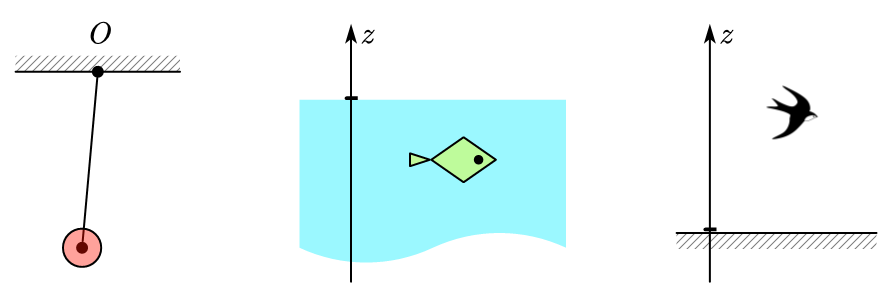
\includegraphics[width=14cm]{image/6-2-1.png}
\caption{可解约束}
\end{figure}

其中,\,	小球的位置符合$x^2+y^2+z^2\leq l^2$,\,鱼的位置符合$z\leq 0$,\,鸟则是$z\geq 0$.

更简单的例子还包括两个物体表面发生接触(滑动或滚动)的情况.\,此时两物可能会脱离接触,\,比如在半球面顶点上滑下来的质点.\,这些所有约束的典型特点,\,从约束方程上看都是一个单边不等式:
\[F\geq 0\quad {\rm or}\quad F\leq 0\]

如果不等式取等号,\,那么可以认为对物体运动的限制客观存在,\,从而会相伴相生约束力.\,但是如果运动到不等号成立了,\,比如上面三种情形中,\,绳子松弛了,\,鱼没有在表面游鸟也没有在地面走,\,那么其实原则上也不存在任何对运动的限制.\,称作约束被``解除''了.\,所以单边约束也可以称作可解约束.\,显然为了简单起见,\,我们可以把这一类问题分解为严格符合约束和没有约束两种情形来等效.\,这实际上构成了不可解的\emph{双边约束}(bilateral constraint)模型.

所谓双边约束就是把之前的单边的约束的不等式进行等式化,\,比如$x^2+y^2+z^2= l^2$就对应着把可弯曲的轻绳替换为了不可弯曲的轻杆.\,而后两个问题就变成了$z=0$,\,即不能让物体陷入也不能让物体脱离的平面约束.

故,\,针对这一类分类模式,\,双边约束显然才是``有效''的部分.\,故本书以后所有约束都指双边的.

继续根据约束的不同特点分类,\,我们就产生了两种可行的依据与分法:

一是,\,根据约束的可积性来分为\emph{完整约束}(holonomic constraint)和\emph{非完整约束}(nonholonomic constraint).

我们发现,\,一个体系的运动由若干\emph{广义坐标}(general coordinates)和它们的导数---\emph{广义速度}(general velocity)来描述.\,比如一个转盘就可以由转角$\varphi$来描述其处在的几何位置\footnote{注意,\,$\varphi$与$\varphi+2\pi$描述的位置在几何上没有区别,\,仅仅是在运动的不同过程中发生,\,一般认为达到后一个位置就是回到了初始位置(运动经历一个周期).},\,而角速度$\dot{\varphi}$来描述转动快慢.\,从而约束,\,作为对运动的限制,\,也就是应当关于这些量的方程.

但是无可辩驳的是,\,在约束发生时这一类方程,\,至少在最初被确定下来的形式下分为两大类,\,一是不含广义速度的\emph{几何约束}(geometric constraint),\,二是含广义速度的\emph{微分约束}(differential constraint).

举三个例子:

A.\,一个圆盘状的冰球本来由盘心的$(x,\,y,\,z)$和盘面方向,\,即垂直盘面的单位法向量$(\cos\alpha,\,\cos\beta,\,\cos\gamma)$构成其广义坐标,\,后面的描述方法用到了方向余弦.\,即使盘并没有被地面约束,\,三个方向余弦也要满足:
\[\cos^2\alpha+\cos^2\beta+\cos^2\gamma=1\]

现在盘到了地面(光滑冰面)上,\,更是要满足:
\[z=0\quad,\quad \alpha=\beta=\frac{\varphi}{2}\quad,\quad \gamma=0\]

这些都是几何约束.

B.\,一个半径为$R$的轮子沿$x$方向单纯地在地面做纯滚动.\,本来在没有地面之前,\,轮子由水平竖直坐标$(x,\,z)$以及自转角$\varphi$描述.\,但是,\,在有了地面做约束以后,\,就需要满足接触条件和纯滚条件(第一章学过):
\[z=0\quad ,\quad \dot{x}=R\dot{\varphi}\]

第一个约束是几何约束,\,第二个便是微分约束.

\begin{wrapfigure}[17]{o}[-10pt]{5cm}
\centering

\includegraphics[width=5cm]{image/6-2-6.jpg}
\caption{独轮车}
\end{wrapfigure}
C.\,考虑一个踩着独轮车在地面上运动的小丑,\,并忽略运动的一些细节,\,认为小丑仅仅由其水平面上坐标$(x,\,y)$和面朝方向$\theta$描述.\,且要求轮子在地面上做纯滚动,\,轮子滚动方向就是小丑面朝方向.\,描述轮子还需已知自转角$\varphi$,\,轮子半径依然为$R$.\,这些就是描述这个体系的所有广义坐标.\,那么客观地看这里有两个限制关系:
\[\frac{\dot{y}}{\dot{x}}=\frac{\sin\theta}{\cos\theta}\quad,\quad \sqrt{\dot{x}^2+\dot{y}^2}=R\dot{\varphi}\]

两个都是实打实的微分约束.

之所以称作微分约束,\,往往是因为这些约束一般都可以对广义速度齐次化,\,尤其是可以一次齐次化,\,B中的例子已经是关于广义速度$\dot{x},\,\dot{\varphi}$的一次线性组合等式了,\,C的例子也可以化为:
\[\dot{x}=R\cos\theta\dot{\varphi}\quad,\quad \dot{y}=R\sin\theta\dot{\varphi}\]

这样我们就可以在等号左右同时乘以$\ud t$,\,写成对各个变量变化微元之间的``约束''或``限制'':
\[{\rm Case\; B}:\quad \ud x=R\ud \varphi\]
\[{\rm Case\; C}:\quad \ud x=R\cos\theta\ud \varphi\quad;\quad \ud y=R\sin\theta\ud \varphi\]

这样就避免了广义速度的引入,\,依然是广义坐标之间的制约关系,\,只不过各个量不全是坐标本身,\,还含有当下状态到下一个状态间坐标的微分.

那么约束的完整性也以上两种约束是什么关系?\,我们需要注意到,\,在B中的那个约束其实是可以积分的.\,约束方程的成立就意味着:
\[x-R\varphi=x(0)-R\varphi(0)={\rm Const.}\]

这样岂不就退化为几何约束了吗?\,的确,\,像这样的微分约束与一个几何约束``等效''.\,从而我们把几何约束和可以用微分约束等效出来的几何约束一同称作完整约束.\,如果一个体系内所有约束都是完整约束,\,那么这样的体系称作\emph{完整体系}(holonomic system).\,后面我们就会发现,\,分析力学中的很多主要结论都有体系必须是完整体系的要求.

反之,\,C就不是一个完整体系了,\,因为体系含有不可积分的微分约束.\,任何看出这一点来的?\,设想通过某种积分的方式我们得到了体系的一个几何约束:
\[F(x,\,y,\,\theta,\,\varphi)=0\]

这蕴含的结果马上就会招致一个矛盾.\,对于几何约束,\,例如在B中的后一个化为的$x-R\varphi={\rm Const.}$,\,总是有经历一个复杂的过程如果$x$复原了,\,$\varphi$也会随之复原.\,这里也一样,\,如果假定以上几何约束存在,\,$F$至少``真正''含有$(x,\,y,\,\theta,\,\varphi)$四个变量之一,\,不妨设是$\varphi$\footnote{其它可能性请读者自己琢磨.}.\,那么如果在一个过程中$x,\,y,\,\theta$均复原,\,那么前后都满足约束方程的话$\varphi$一般就只有有限个解,\,更特殊地,\,必然要求也回到初态发生复原.\,然而,\,联系一下实际的物理情景便可以明白,\,小丑完全有能力让自己的位置回到初始位置,\,面朝方向也归位,\,同时轮子转过一个任意大小的角度的:\,只需要沿着半径或大或小的圆周转圈即可.\,从这一点上我们就可以发现这样的约束是不可能积分化为几何约束的非完整约束.

进一步观察我们还能发现,\,在C问题中$(x,\,y,\,\theta,\,\varphi)$四个变量具有某种``全局独立性'',\,我们总是有办法把任意的两个$(x_1,\,y_1,\,\theta_1,\,\varphi_1),\,(x_2,\,y_2,\,\theta_2,\,\varphi_2)$作为初末态用过程进行连接.\,但是我们决不要因此而认为这几个变量之间因此就彼此独立不会相互制约,\,因为约束方程客观存在,\,也就是说,\,考虑任一个状态下一时刻发生的位移$(\ud x,\,\ud y,\,\ud \theta,\,\ud \varphi)$,\,它们在``局域''看来并不具有独立性而是有相关性.\,这种\emph{局部处处成立}(locally holds everywhere)但\emph{全局不生效}(globally invalid)的行为是出于较深刻的拓扑学和分析学的原因\footnote{位形-微分流形上约束对应的矢量场间具有不为零的李导数.}.\,需要加以留心.

第二种分类方式则更加清晰明了.\,它取决于约束方程本身含不含时.\,例如在之前的绳端系球,\,以及在上面的C中的一约束方程中:
\[x^2+y^2+z^2=l^2 \quad;\quad \ud x=R\cos\theta\ud \varphi\]

它们都是不含时间的.\,从而称为\emph{稳定约束}(scleronomic constraints)\footnote{来自希腊语``坚硬'':  \begin{greek} skle'os\end{greek}}.\,但是它们对应着还存在类似的,\,\emph{非稳定约束}(rheonomic constraints)\footnote{来自希腊语``流动'':  \begin{greek} <r'ew\end{greek}}的版本,\,一种可能的情况如下:
\[x^2+y^2+z^2=(l+vt)^2 \quad;\quad \ud x=(R+vt)\cos\theta\ud \varphi\]

它们就表示绳子还在不断变长或者轮子半径在不断膨胀的新的问题.

与之前的完整非完整体系造成的区别不同,\,也许在牛顿的力学体系中处理一个非完整约束体系和非稳定约束体系的难度是相当的:\,都要进行细致的受力分析,\,能量守恒不成立或者虽然成立但用处不大.\,但是在分析力学中,\,一个体系即使约束非稳定也是与稳定约束一样适用于大多数结论的.\,分析力学的方法在求解非稳定但完整的理想约束体系中是一大利器.

\subsection{广义坐标与自由度}

拥有了约束的观点,\,便很好理解广义坐标之间的独立性的概念.\,\emph{自由度}(DOF,\,degree of freedom)也正是基于这一点而产生.\,它的定义是:\,考虑所有约束条件都成立的前提下,\,体系可以独立改变的坐标微分个数.

一般来说,\,在三维空间中(以下所有结论在二维或高维空间中都得重新讨论),\,在把一个体系的所有存在的约束都完全解除之后,\,体系可能由质点,\,线状刚体或者非线状刚体组成.\,那么直接地我们给出或者规定:\,质点的自由度为3,\,非线状刚体的自由度为6,\,线状刚体的自由度为5.\,这一点待会就可以验证.\,而一个体系若包含$a$个质点,\,$b$个线状刚体,\,$c$个非线状刚体.\,而如果约束的引入为体系带来了$r$个独立的约束方程(几何约束或微分约束),\,显然根据自由度的定义,\,体系独立变化的广义坐标的数目降为:
\[s=3a+5b+6c\quad \longrightarrow \quad f=s-r\]

这个$f$就是最终的自由度的个数.

质点的自由度为3自然是最好理解的.\,无论是用直角坐标,\,球坐标还是柱坐标,\,互相独立的坐标个数都是3.\,而它们之间又不存在任何制约关系.

如果我们把两个质点用一个刚性棍连接,\,就会带来一个距离不变的约束.\,体系自由度变为:
\[f=2\cdot 3-1=5\]

这实际上就是线状刚体的自由度数.\,因为只要确定好线状刚体上的两个点的$6$个坐标,\,那么实际上就构成了对刚体的完整描述:\,每一个质元的位置都可以简单找到.\,而这六个坐标又有一个约束关系,\,从而自由度为5.

但是非线状刚体就更复杂.\,既然非线状必然能够在刚体上找到三个不共面的固连点.\,只要确定好这三个点的9个坐标就能确定整个刚体的位形.\,但是这三个点之间两两距离不变,\,存在三个独立的约束方程,\,所以自由度数变为:
\[f=9-3=6\]

\begin{wrapfigure}[13]{o}[-10pt]{7cm}
\centering
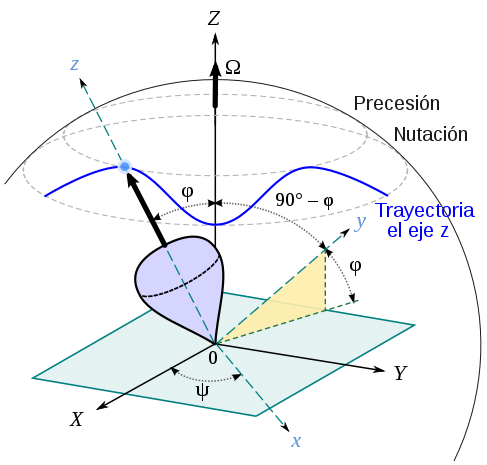
\includegraphics[width=7cm]{image/6-2-2.png}
\caption{刚体的三自由度转动}
\end{wrapfigure}
为什么线状刚体不能作为非线状刚体的特例而也具有相同的6自由度呢?\,比如一个陀螺,\,作为一个刚体分析一般为认为它有三个平动自由度和三个转动自由度.\,如果陀螺做定点转动,\,它的三个转动自由度就被简单地隔离了出来:\,它们是自转,\,进动和章动.\,但是我们不能指望一根线状刚体来自转:\,自转进行一个角度,\,对应的状态却实际上与之前的状态没有本质区别.\,更重要地是反映在能量上,\,自转既没有带来动能,\,也没有带来势能的改变,\,从而自转角根本就是一个冗余的\emph{内禀自由度}(intrinsic DOF),\,不会参与问题的讨论过程中.

从而以上论断也将基于一个基本事实:\,质点和线状刚体是真正理想的,\,现实模型:\,小球,\,细棍更精细的模型当然是6自由度的刚体,\,甚至更高自由度的质点系,\,连续体模型.

清楚了体系的基本组成部分的原始自由度数.\,我们再把视野转向常见的约束上来.

要注意,\,约束的个数这样一种说法的歧义性.\,有时候我们发现体系有$r$个独立的约束方程,\,从而说体系存在$r$个约束.\,但是有时候我们指的是有几个机构在制约着物体的运动.\,两者是有区别的,\,我们保留前者的称呼,\,后者的个数叫做约束物的个数.

Case1.\,如果用一个面来限制质点的运动,\,那么约束的个数是1.\,如果质点是一颗珠子被穿在一条空间曲线上,\,那么尽管约束物只有一个,\,但存在两个约束.\,这是因为平面和曲线方程分别是:
\[{\rm Surface:} \quad F(x,\,y,\,z)=0 \quad;\quad {\rm Curve:} \quad \left\{ \begin{matrix} F(x,\,y,\,z)=0\\ G(x,\,y,\,z)=0\end{matrix}\right.\]

这也正构成了两种情况下的约束方程.
\begin{figure}[H]
\centering
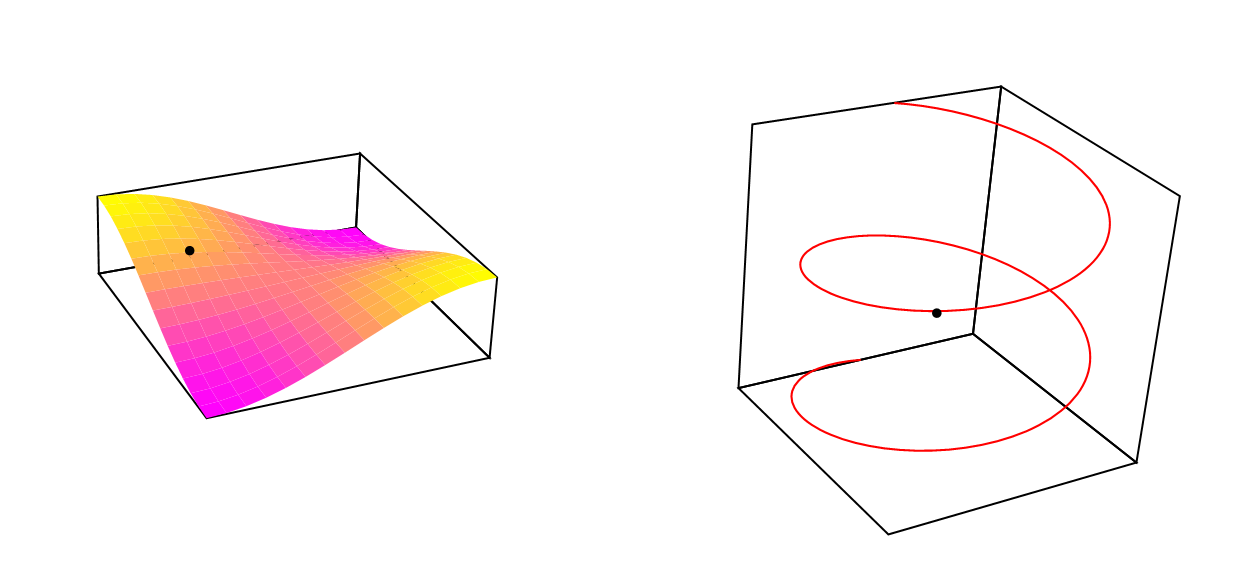
\includegraphics[width=14cm]{image/6-2-3.png}
\caption{面约束和线约束}
\end{figure}

Case2.\,但是,\,如果面和线是绝对粗糙的,\,那么质点就动弹不得.\,这样带来的约束个数,\,显然两种情况都有三个.

Case3.\,用绳子和杆子的两端连接两个物体,\,对应的约束个数显然是1.\,就是说那两个点之间的距离为一个常数.

Case4.\,如果绳子还绕过了滑轮,\,那么原则上每一段绳带来一个约束减少一个自由度.\,例如坐标为$(x_1,\,y_1,\,z_1)$的质点连接的绳(长$l$)绕过坐标为$(x_2,\,y_2,\,z_2)$的滑轮(视作质点)与坐标为$(x_3,\,y_3,\,z_3)$的质点连接,\,约束方程就是:
\[\sqrt{(x_2-x_1)^2+(y_2-y_1)^2+(z_2-z_1)^2}+\sqrt{(x_2-x_3)^2+(y_2-y_3)^2+(z_2-z_3)^2}=l\]

Case5.\,而不同于用两段绳分别连接12和23,\,这样就会带来两个约束.\,区别在于前者的一段绳两个部分可以交换绳长,\,但是后者的两段绳则不能交换绳长.

Case6.\,最后还有铰链模型.\,如果仅仅是两个物体用铰链连接,\,那么结论是显然的:\,如果是平面问题,\,那么约束个数为2.\,如果是空间问题,\,那么约束个数为3.\,约束方程就是被连接的两个点具有完全一致的所有坐标.

Case7.\,但如果是$n$个物体同时连接与一个铰链上,\,那么我们只需要把第1个物体和第2个物体连接,\,再把第2个物体和第3个物体连接...\, 最终把第$n-1$个物体同第$n$个物体连接即可,\,一共进行了$n-1$次独立的连接,\,故约束个数为$2(n-1)$(平面问题)或$3(n-1)$(空间问题).
\vspace{1cm}

引入自由度的概念,\,一个重要的原因是为了更好地描述体系的运动.\,现在我们先看更复杂的情况:\,如果体系是非完整体系,\,那么事情比较难办:\,不妨设$r$个独立约束中应当有$h$个完整约束和$k$个不完整的约束.\,那么应当给予保留$f'=s-h$个广义坐标.\,体系的运动过程中,\,这$f'$个广义坐标并不能完全相互决定,\,记作$q_1,\,q_2\cdots q_{f'}$.\,但是体系任意状态的描述都只需要确定这$f'$个广义坐标的值和导数.\,比如,\,任何一个质点的$x$坐标,\,还有速度的$x$分量就必然可以用之前的量来表示.\,而还应当存在$k$个微分约束:
\[x=x(q_i,\,t)\quad,\,\quad \dot{x}=\frac{\partial x}{\partial t}+\sum_i \frac{\partial x}{\partial q_i}\dot{q_i}\]
\[f_j(q_i,\,\ud q_i,\,\ud t)=0\]
\[i=1,\,2\cdots f' \quad,\quad j=1,\,2\cdots k\]

但是如果是完整体系,\,问题就简单了,\,自由度的个数$f$就会是体系独立的坐标的个数.\,从而如果广义坐标是$q_1,\,q_2\cdots q_f$,\,它们之间就不存在约束关系了,\,体系的一切量,\,原来如果由类似于$x,\,\dot{x}$这样的量来表示,\,现在就直接是:
\[x=x(q_i,\,t)\quad,\,\quad \dot{x}=\frac{\partial x}{\partial t}+\sum_i \frac{\partial x}{\partial q_i}\dot{q_i}\quad (i=1,\,2\cdots f)\]

尤其是稳定的完整约束体系.\,那么由于约束方程不含$t$,\,那么上式就更是简化为:
\[x=x(q_i)\quad,\,\quad \dot{x}=\sum_i \frac{\partial x}{\partial q_i}\dot{q_i}\quad (i=1,\,2\cdots f)\]



\subsection{约束力与广义力}

为了简单起见,\,我们把刚体也当作多个通过约束固连在一起的质点构成的系统.\,这样体系便只含有以下要素:\,质点,\,外力,\,约束,\,质点间的内力,\,约束力(也是内力).

正过来看,\,任何一个约束都可以限制到若干质点.\,从而同时对这几个物体的运动提出单个的制约关系(自由度减1).

但是另一方面,\,每一个质点又同时可能受到若干个约束物的共同限制,\,每一个约束物就会对该质点施加一个或多个约束方程来把这个质点的运动和其他质点运动联系起来.

在牛顿力学情况下,\,我们总是喜欢分析那个质点受到的约束物给它的力的具体特征.\,这种力就叫做约束力.

约束力的最核心特征,\,就在于它是\emph{被动力}(passive force).\,直接看是找不到这么一个力的大小与方向的.\,约束力的具体值,\,是两个因素共同作用的结果:\,一方面就是约束本身的性质:\,是光滑的还是粗糙的?\,是要耗散还是甚至可以输出能量?\,但是更重要的是,\,约束力必然受到具体运动情况和体系动力学结构的影响.\,这一点很好理解:\,因为如果把某个约束解除,\,那么体系之后的运动就不一定遵从约束方程.\,那么解除约束之前的体系就正是因为约束给出来的力影响了其运动而导致其运动``回归正轨''.

基于这一点,\,就不难判断,\,质点受到``必要''约束力的个数,\,就是质点坐标参与约束方程的个数.

比如,\,被穿在光滑曲线上的质点受到的约束力必然是两个,\,再比如,\,平面问题中,\,两个用光滑铰链连接的物体会在两个方向上产生约束力,\,而如果是$n$个物体铰接在一起,\,那么期间我们如果设出$2(n-1)$个约束力就意味着个数设对了.


显然,\,如果是粗糙的曲线上有一个滑动的质点,\,曲线给质点的力应当有两个支持力和一个滑动摩擦力,\,也就是说应当是三个,\,而不是约束给出的两个.\,再比如,\,将一条长$l$的轻绳子绕过三个光滑滑轮组成一个闭合的圈.\,那么明显每个物体与之相关的约束方程只有一个.\,但是约束力似乎也得有两个拉力.

\begin{wrapfigure}[13]{o}[-10pt]{5cm}
\centering
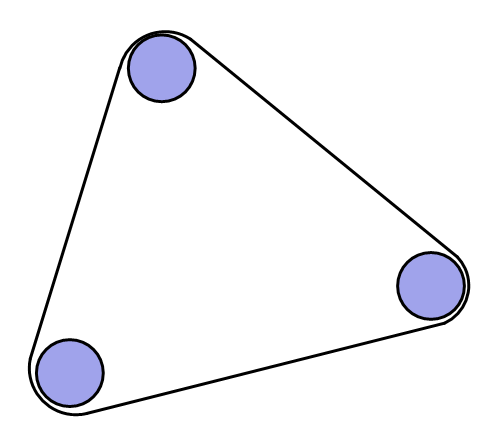
\includegraphics[width=5cm]{image/6-2-4.png}
\caption{三物体一约束}
\end{wrapfigure}
这两种情况也得分开讨论.\,第二种情况下,\,两个拉力总是相等,\,从而三个质点的受力都指向三个角平分线的交点:\,内心.\,这个约束给三个质点的力其实应当认为是两个力的合力.\,它只有沿内心与质点连线方向的分量,\,没有垂直方向的,\,可以算作一个约束力而不是两个.\,但是前者的确应当算作三个约束力.\,这是因为滑动摩擦力分量明显不是``必要的''.\,它独立于之前的两个支持力.\,也不同于之前两个支持力.

其中具体的道理还得见后面虚功原理一节的关于理想约束的推导.\,我们指出,\,在上一章讨论约束力功的时候我们提出的约束力公式,\,在这里可以直接推广.\,实际上就能得到我们一直在说的``必要''约束力.\,在一般情况下,\,如果某约束对一质点的$x$坐标产生了限制:
\[f(x,\cdots)=0\]

那么与之相伴而生的作用在质点上的约束力就必然有一项$x$分量:
\[F_x=\lambda_f\frac{\partial f}{\partial x}\]

如果还含$y$那$y$方向自然也会产生一个约束力,\,公式是一样的.\,如果含有其他质点坐标时就换那个质点的坐标来求片导数.\,注意由同一个约束方程产生的所有的约束力都共用同一个$\lambda_f$.

对于理想约束这就是全部的约束力和它要符合的形式,\,非理想约束则可能产生各种各样的其它形式的约束力.

还有一个重要概念需要先一步加以介绍.\,如果我们考虑任何一个作用在实际体系的某质点上的力$\bs{F}$,\,该质点坐标为$\bs{r}=(x,\,y,\,z)$.\,我们引入一个新的概念.\,这个力产生的在每一个广义坐标$q_i$上的广义力$Q_i$:\,其定义也相当简单,\,就是要使得下面连等式成立:
\[\ud W=\bs{F}\cdot \ud \bs{r}=\sum_i Q_i\ud q_i\]

这是希望用广义力对广义位移来做功来代替以往的矢量力对质点做功的一成不变的做法.\,我们默认体系都是稳定约束,\,那么其实该质点的任意位移,\,简单地可以用广义坐标上的位移来表示:
\[\bs{r}=\bs{r}(q_i)\quad \Rightarrow \quad \ud \bs{r}=\frac{\partial \bs{r}}{\partial q_i}\ud q_i\]

代入之前的要求就发现,\,广义力的算法为:
\[Q_i=\bs{F}\cdot\frac{\partial \bs{r}}{\partial q_i}\]
\vspace{0.5cm}

\begin{wrapfigure}[13]{o}[-10pt]{4cm}
\centering
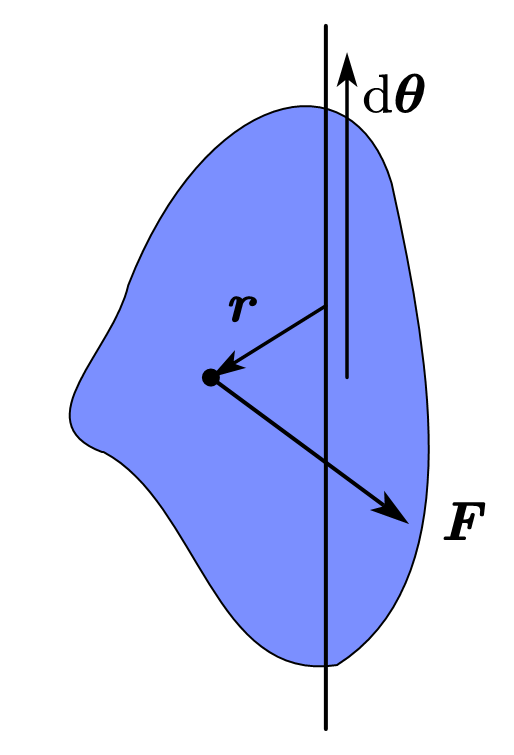
\includegraphics[width=4cm]{image/6-2-5.png}
\caption{力矩作为广义力}
\end{wrapfigure}
举两个例子:

一是刚体可做定轴转动,\,那么当刚体产生$\ud \bs{\theta}=\ud \theta \bs{e}$的转动时,\,作用在$\bs{r}$的力$\bs{F}$的作用点的实际位移为:
\[\ud \bs{r}=\ud \bs{\theta}\times \bs{r}\]

那么力的实际做功为:
\begin{align*}
\ud W  &=\bs{F}\cdot \ud \bs{r}\\
		    &=\bs{F}\cdot(\ud \bs{\theta}\times \bs{r})\\
			&=(\bs{r}\times\bs{F})\cdot\ud \bs{\theta}\\
			&=\bs{M}\cdot \bs{e}\ud \theta\\
			&=Q_\theta \ud \theta
\end{align*}

这也就是说,\,沿轴方向的力矩$\bs{M}\cdot \bs{e}$就是与角位移$\ud \theta$伴随的广义力$Q_\theta$.

\begin{wrapfigure}[17]{o}[-10pt]{3cm}
\centering
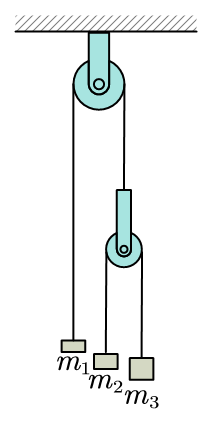
\includegraphics[width=3cm]{image/6-2-7.png}
\caption{滑轮组}
\end{wrapfigure}
再来看看在牛顿力学体系中比较基础的滑轮组问题.\,如果两个自由度分别取为:\,一.\,2,\,3挂着的动滑轮的下降与1上升的高度x;\,二.\,相对动滑轮,\,2的上升与3的下降高度y.\,那么1,\,2,\,3的向下位移就分别为:
\[s_1=-x\quad,\quad s_2=x-y\quad,\quad s_3=x+y\]

这样,\,三个重力在这两个自由度上累积的广义力就是:
\[Q_x=-m_1g+(m_2+m_3)g\]
\[Q_y=(m_3-m_2)g\]

这有什么用?\,实际上我们计算动能还可以得到``广义质量'':
\begin{align*}
T 	&=\frac{1}{2}(m_1\dot{s}_1^2+m_2\dot{s}_2^2+m_3\dot{s}_3^2)\\
	&=\frac{1}{2}(m_1+m_2+m_3)\dot{x}^2+\frac{1}{2}(m_2+m_3)\dot{y}^2+(m_3-m_2)\dot{x}\dot{y}
\end{align*}


其实这个广义力乘广义位移等于做功的现象我们并不少见,\,不管是热学中的$\ud W=-p\ud V$,\,还是电路问题中的$\ud W=U\ud Q$,\,抑或是电磁介质问题中的$\ud W=E\ud P,\,\ud W=H\ud M$等等公式.\,全都归于统一的广义力乘广义位移这样的形式上.\,

\section{力系化简}

静力学中大量涉及到由质点,\,刚体和简单约束构成的问题.\,本节正是要针对这一类问题形成行之有效的强大工具.\,我们建立在之前的理论基础上,\,重新构建静力学过程中适用的新公理体系.

\subsection{公理化静力学体系}



\subsection{力系向一点简化}

一

\section{平衡问题:\,矢量力学}

\subsection{平衡问题的要素}

一

\subsection{平衡条件与判据}

一

\subsection{负静定,\,静定与超静定}

一

\subsection{静摩擦的临界}

一

\section{平衡问题:\,虚功原理}

\subsection{理想约束}

一

\subsection{负静定问题的虚功原理}

一

\subsection{静定,\,超静定问题的求解}

一

\section{分析力学初步*}

\subsection{用广义坐标表示能量}

一

\subsection{拉格朗日方程}

一

\subsection{再论冲击问题}

一

\subsection{哈密顿力学简介}

一

\section{平衡态稳定性}

\subsection{一自由度体系}

一

\subsection{多自由度体系}

一
